\documentclass[12pt, A4]{article}\usepackage[]{graphicx}\usepackage[]{color}
%% maxwidth is the original width if it is less than linewidth
%% otherwise use linewidth (to make sure the graphics do not exceed the margin)
\makeatletter
\def\maxwidth{ %
  \ifdim\Gin@nat@width>\linewidth
    \linewidth
  \else
    \Gin@nat@width
  \fi
}
\makeatother

\definecolor{fgcolor}{rgb}{0.345, 0.345, 0.345}
\newcommand{\hlnum}[1]{\textcolor[rgb]{0.686,0.059,0.569}{#1}}%
\newcommand{\hlstr}[1]{\textcolor[rgb]{0.192,0.494,0.8}{#1}}%
\newcommand{\hlcom}[1]{\textcolor[rgb]{0.678,0.584,0.686}{\textit{#1}}}%
\newcommand{\hlopt}[1]{\textcolor[rgb]{0,0,0}{#1}}%
\newcommand{\hlstd}[1]{\textcolor[rgb]{0.345,0.345,0.345}{#1}}%
\newcommand{\hlkwa}[1]{\textcolor[rgb]{0.161,0.373,0.58}{\textbf{#1}}}%
\newcommand{\hlkwb}[1]{\textcolor[rgb]{0.69,0.353,0.396}{#1}}%
\newcommand{\hlkwc}[1]{\textcolor[rgb]{0.333,0.667,0.333}{#1}}%
\newcommand{\hlkwd}[1]{\textcolor[rgb]{0.737,0.353,0.396}{\textbf{#1}}}%
\let\hlipl\hlkwb

\usepackage{framed}
\makeatletter
\newenvironment{kframe}{%
 \def\at@end@of@kframe{}%
 \ifinner\ifhmode%
  \def\at@end@of@kframe{\end{minipage}}%
  \begin{minipage}{\columnwidth}%
 \fi\fi%
 \def\FrameCommand##1{\hskip\@totalleftmargin \hskip-\fboxsep
 \colorbox{shadecolor}{##1}\hskip-\fboxsep
     % There is no \\@totalrightmargin, so:
     \hskip-\linewidth \hskip-\@totalleftmargin \hskip\columnwidth}%
 \MakeFramed {\advance\hsize-\width
   \@totalleftmargin\z@ \linewidth\hsize
   \@setminipage}}%
 {\par\unskip\endMakeFramed%
 \at@end@of@kframe}
\makeatother

\definecolor{shadecolor}{rgb}{.97, .97, .97}
\definecolor{messagecolor}{rgb}{0, 0, 0}
\definecolor{warningcolor}{rgb}{1, 0, 1}
\definecolor{errorcolor}{rgb}{1, 0, 0}
\newenvironment{knitrout}{}{} % an empty environment to be redefined in TeX

\usepackage{alltt}
%\usepackage[brazil]{babel}
\usepackage{graphicx}
\usepackage[utf8]{inputenc}
\usepackage[T1]{fontenc}
\usepackage{url}
\usepackage{natbib}
\bibliographystyle{rusnat}
\usepackage{framed, color}
\usepackage{xspace}
\definecolor{shadecolor}{rgb}{0.9, 0.9, 0.9}
\newcommand{\R}{\textnormal{\sffamily\bfseries R}\xspace}
\newcommand{\code}[1]{\texttt{#1}}


\title{Parametric estimates of total tree richness in Amazon}
\author{Han Ter Steege, Paulo Inácio Prado, Renato Lima, ATDN}
\IfFileExists{upquote.sty}{\usepackage{upquote}}{}
\begin{document}

\maketitle




\begin{knitrout}
\definecolor{shadecolor}{rgb}{0.969, 0.969, 0.969}\color{fgcolor}\begin{kframe}
\begin{alltt}
\hlstd{dados} \hlkwb{<-} \hlkwd{read.csv2}\hlstd{(}\hlstr{"data.csv"}\hlstd{,} \hlkwc{as.is}\hlstd{=}\hlnum{TRUE}\hlstd{)}
\hlstd{y} \hlkwb{<-} \hlstd{dados}\hlopt{$}\hlstd{N.ind}
\hlstd{Sobs} \hlkwb{<-} \hlkwd{length}\hlstd{(y)}
\hlcom{## Total number of trees (average density x area)}
\hlstd{Tot.t} \hlkwb{<-} \hlnum{567}\hlopt{*}\hlnum{5.5e8}
\hlcom{## Proportion of total trees in the sample}
\hlstd{p1} \hlkwb{<-} \hlkwd{sum}\hlstd{(dados}\hlopt{$}\hlstd{N.ind)}\hlopt{/}\hlstd{Tot.t}
\hlcom{## Total number of plots}
\hlstd{N.plots} \hlkwb{<-} \hlnum{1945}
\end{alltt}
\end{kframe}
\end{knitrout}

\section*{Poisson lognormal}

Seems to overestimate the abundance of the most abundant species (see qq-plots)
 
\begin{knitrout}
\definecolor{shadecolor}{rgb}{0.969, 0.969, 0.969}\color{fgcolor}\begin{kframe}
\begin{alltt}
\hlstd{pln} \hlkwb{<-} \hlkwd{fitpoilog}\hlstd{(y)}
\hlkwd{par}\hlstd{(}\hlkwc{mfrow}\hlstd{=}\hlkwd{c}\hlstd{(}\hlnum{2}\hlstd{,}\hlnum{2}\hlstd{))}
\hlkwd{plot}\hlstd{(pln)}
\hlkwd{par}\hlstd{(}\hlkwc{mfrow}\hlstd{=}\hlkwd{c}\hlstd{(}\hlnum{1}\hlstd{,}\hlnum{1}\hlstd{))}
\end{alltt}
\end{kframe}

{\centering 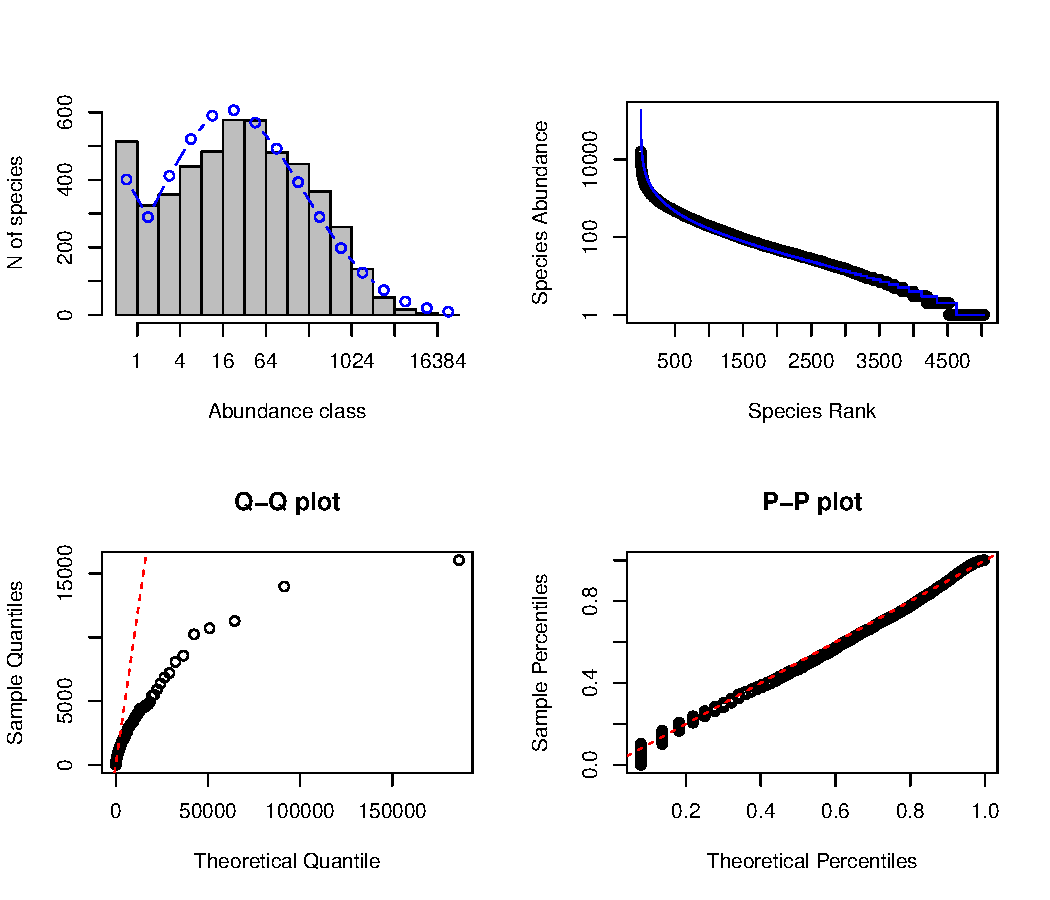
\includegraphics[width=\maxwidth]{figure/fit_pln-1} 

}



\end{knitrout}

\subsection*{Species richness estimation from the underlying lognormal}


Still, let's use the estimated coefficients to estimate total species richness.
The estimated parameters of the Poilog are:

\begin{knitrout}
\definecolor{shadecolor}{rgb}{0.969, 0.969, 0.969}\color{fgcolor}\begin{kframe}
\begin{alltt}
\hlstd{(pln.cf} \hlkwb{<-} \hlkwd{coef}\hlstd{(pln))}
\end{alltt}
\begin{verbatim}
##       mu      sig 
## 2.787362 2.491355
\end{verbatim}
\end{kframe}
\end{knitrout}

In this model the observed SADs is a Poisson sample of a lognormal SAD of the whole community.
The parameter $\sigma$ of the Poilog estimates the same parameter of the underlying lognormal.
The parameter $\mu$ of the Poilog has the following relationship with the corresponding parameter
of the sampled lognormal ($M$):

$ M = \mu - \ln(p)$

where $p$ is the proportion of the community that has been sampled
\citep{Bulmer1974,Saether2013}.
%% As the total sampled area is $2.048 \times 10^3$ ha and the 
%% total area of Amazon is $5.79 \times 10^8$ ha, $p=$~(p1=2.048e3/5.79e8).
%% Therefore, we have $M=$~unname(pln.cf[1])-log(p1).

As the estimated total number of trees in  Amazon is $3.1 \times 10^{11}$, 
and the number of identified trees in the sample
is 986577, $p=$~\ensuremath{3.1636267\times 10^{-6}}.
Therefore, we have $M=$~15.4511534.

The mean of the lognormal distribution is 

$E[X] = e^{M + \frac{\sigma^2}{2}}$

And then this model says that the regional SAD is lognormal
with an average number of trees/species of

 
\begin{knitrout}
\definecolor{shadecolor}{rgb}{0.969, 0.969, 0.969}\color{fgcolor}\begin{kframe}
\begin{alltt}
\hlstd{pln.cf} \hlkwb{<-} \hlkwd{unname}\hlstd{(pln.cf)}
\hlstd{Mu} \hlkwb{<-} \hlstd{pln.cf[}\hlnum{1}\hlstd{]}\hlopt{-}\hlkwd{log}\hlstd{(p1)}
\hlstd{(mean.ln} \hlkwb{<-} \hlkwd{exp}\hlstd{(Mu} \hlopt{+} \hlstd{pln.cf[}\hlnum{2}\hlstd{]}\hlopt{^}\hlnum{2}\hlopt{/}\hlnum{2}\hlstd{))}
\end{alltt}
\begin{verbatim}
## [1] 114327511
\end{verbatim}
\end{kframe}
\end{knitrout}

The estimated richness is then the total number of trees in the region
divided by the mean above: 

 
\begin{knitrout}
\definecolor{shadecolor}{rgb}{0.969, 0.969, 0.969}\color{fgcolor}\begin{kframe}
\begin{alltt}
\hlcom{## Estimated number of species}
\hlstd{(pln.S} \hlkwb{<-} \hlstd{Tot.t}\hlopt{/}\hlstd{mean.ln)}
\end{alltt}
\begin{verbatim}
## [1] 2727.69
\end{verbatim}
\end{kframe}
\end{knitrout}

Rather disappointing. I guess that the problem is the assumption that the pooled samples
can be approximated by a Poisson sample of the entire tree community of Amazon (pretty unrealistic indeed).


\subsection*{Estimating species richness directly from PLN}

An alternative way \footnote{I guess this is the way recommended by developers of the \emph{poilog} package, to be checked} 
to estimate total number of species in the sampled metacommunity
is simply to calculate the value of the Poisson-lognormal fitted to the data at
the zero value. That is, to estimate the probability value assigned to species that
had zero abundance in the sample. Simple as that:

\begin{knitrout}
\definecolor{shadecolor}{rgb}{0.969, 0.969, 0.969}\color{fgcolor}\begin{kframe}
\begin{alltt}
\hlstd{(pln.d0} \hlkwb{<-} \hlkwd{dpoilog}\hlstd{(}\hlnum{0}\hlstd{,} \hlkwc{mu} \hlstd{= pln.cf[}\hlnum{1}\hlstd{],} \hlkwc{sig}\hlstd{=pln.cf[}\hlnum{2}\hlstd{]))}
\end{alltt}
\begin{verbatim}
## [1] 0.1124546
\end{verbatim}
\end{kframe}
\end{knitrout}

That is, an estimate that the recorded species are 89\%
of the total number of species.
This gives an estimate of 5671 species.

\subsubsection*{Likelihood and confidence intervals}

Confidence profiles for both parameters are quite well-behaved (parabolic)
and so match frequentist confidence intervals:

\begin{knitrout}
\definecolor{shadecolor}{rgb}{0.969, 0.969, 0.969}\color{fgcolor}\begin{kframe}
\begin{alltt}
\hlstd{pln.prf} \hlkwb{<-} \hlkwd{profile}\hlstd{(pln)}
\hlkwd{par}\hlstd{(}\hlkwc{mfrow}\hlstd{=}\hlkwd{c}\hlstd{(}\hlnum{1}\hlstd{,}\hlnum{2}\hlstd{))}
\hlkwd{plotprofmle}\hlstd{(pln.prf)}
\hlkwd{par}\hlstd{(}\hlkwc{mfrow}\hlstd{=}\hlkwd{c}\hlstd{(}\hlnum{1}\hlstd{,}\hlnum{1}\hlstd{))}
\hlstd{(pln.ci} \hlkwb{<-} \hlkwd{confint}\hlstd{(pln.prf))}
\end{alltt}
\begin{verbatim}
##        2.5 %   97.5 %
## mu  2.684205 2.885074
## sig 2.418213 2.569101
\end{verbatim}
\begin{alltt}
\hlstd{(pln.li} \hlkwb{<-} \hlkwd{likelregions}\hlstd{(pln.prf))}
\end{alltt}
\begin{verbatim}
## Likelihood regions for ratio = 2.079442 
## 
##  mu:
##         lower   upper
## [1,] 2.679937 2.88898
## 
##  sig:
##         lower   upper
## [1,] 2.415443 2.57232
\end{verbatim}
\end{kframe}

{\centering 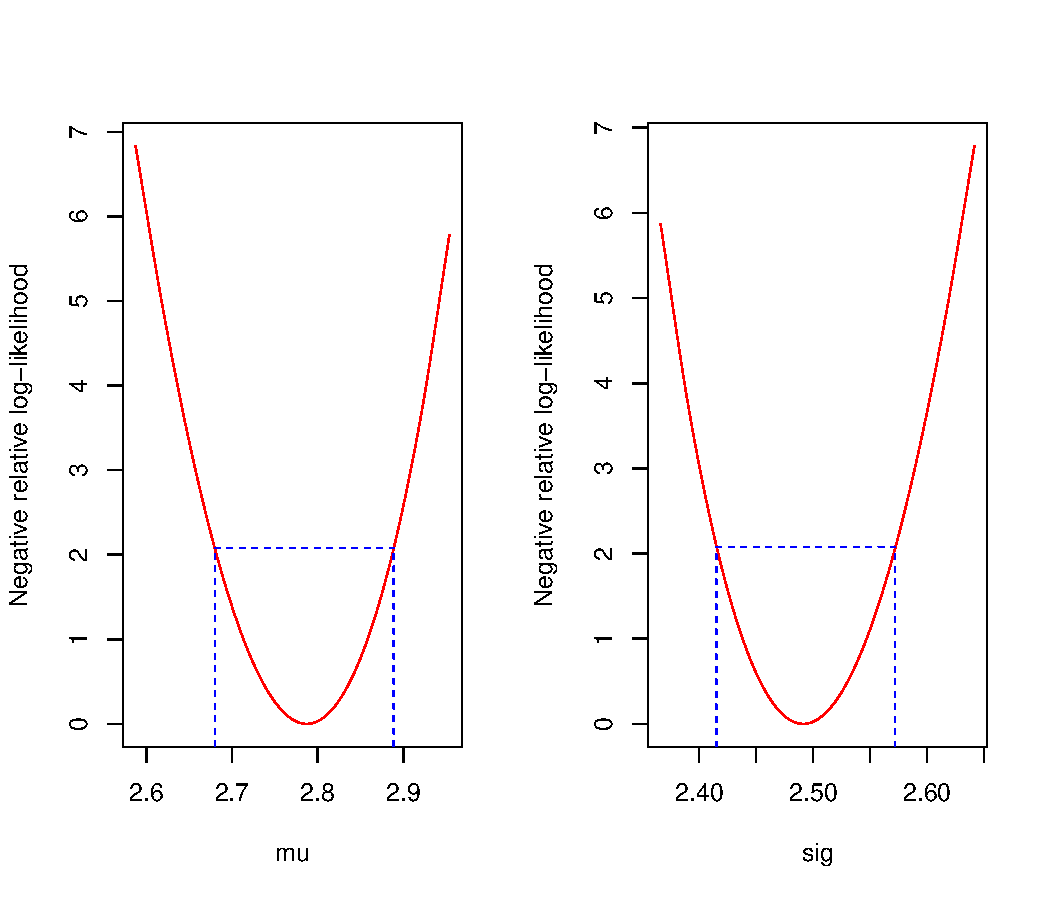
\includegraphics[width=\maxwidth]{figure/confidence_and_likelihood_limits_of_PLN-1} 

}



\end{knitrout}

The likelihood interval of total species richness can be estimated
visually from the likelihood surface. 
Using the likelihood ratio of two (bold black isoline)
we can see the isolines that are tangent tothe likelihood region.
%likelihood interval for total species richness from PLN is ca 5600 -- 5750:

\begin{knitrout}
\definecolor{shadecolor}{rgb}{0.969, 0.969, 0.969}\color{fgcolor}

{\centering 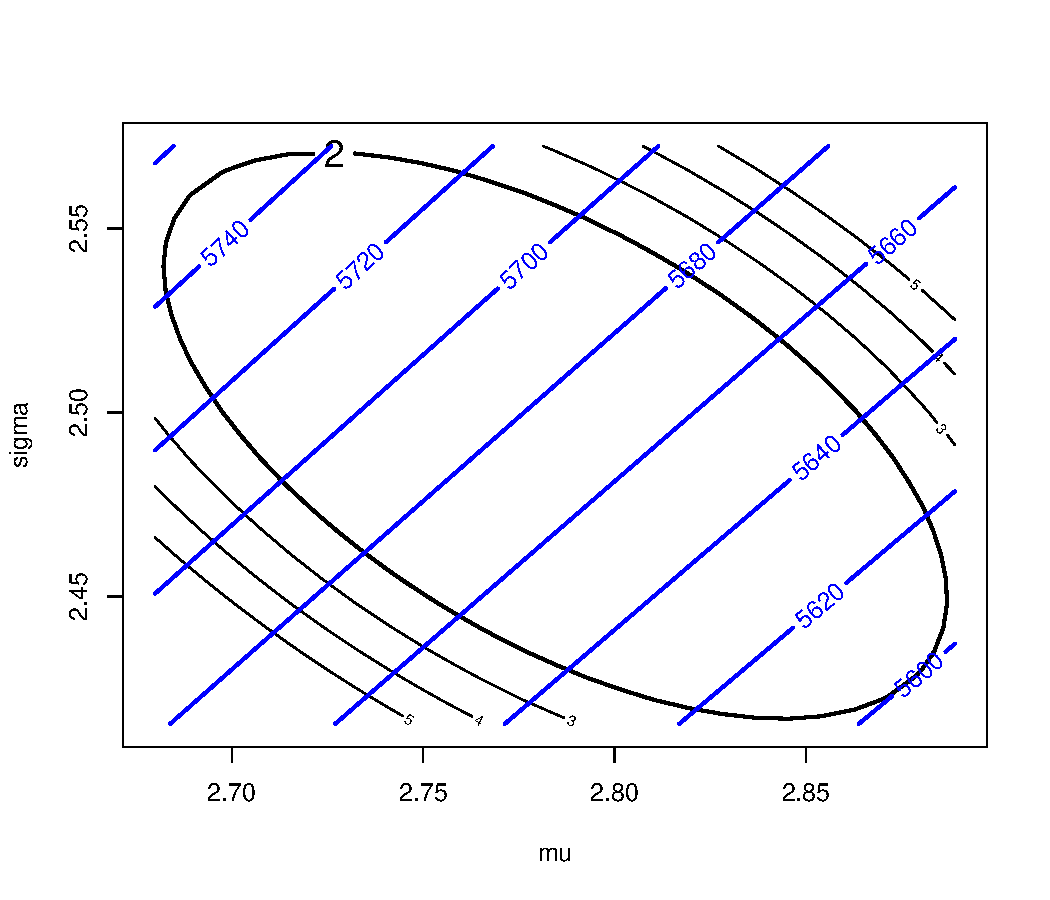
\includegraphics[width=\maxwidth]{figure/PLN_richness_ci-1} 

}



\end{knitrout}

Because confidence intervals of the estimated parameters are very close to likelihood intervals 
we have a similar result using one or another interval to estimate a interval for the total species richness. 
But the likelihood surface help us by showing 
that we have to use the upper bound of $\mu$ CI with the lower bound of $\sigma$ CI
to get the lower bound of species richness (and the opposite for the
upper bound):

\begin{knitrout}
\definecolor{shadecolor}{rgb}{0.969, 0.969, 0.969}\color{fgcolor}\begin{kframe}
\begin{alltt}
\hlcom{## Lower bound of S}
\hlstd{Sobs} \hlopt{/} \hlstd{(}\hlnum{1} \hlopt{-} \hlkwd{dpoilog}\hlstd{(}\hlnum{0}\hlstd{, pln.ci[}\hlnum{1}\hlstd{,}\hlnum{2}\hlstd{], pln.ci[}\hlnum{2}\hlstd{,}\hlnum{1}\hlstd{]))}
\end{alltt}
\begin{verbatim}
## [1] 5592.471
\end{verbatim}
\begin{alltt}
\hlcom{## Upper bound}
\hlstd{Sobs} \hlopt{/} \hlstd{(}\hlnum{1} \hlopt{-} \hlkwd{dpoilog}\hlstd{(}\hlnum{0}\hlstd{, pln.ci[}\hlnum{1}\hlstd{,}\hlnum{1}\hlstd{], pln.ci[}\hlnum{2}\hlstd{,}\hlnum{2}\hlstd{]))}
\end{alltt}
\begin{verbatim}
## [1] 5758.637
\end{verbatim}
\end{kframe}
\end{knitrout}

Still much lower than the estimates provided by log-series or negative binomial.

\section*{Log-series}

Log-series seems to overestimate the number of singletons
and to underestimate the abundance of species with intermediary abundances
(between 16 and 64 individuals, see octave plot). Also, qq-plots show that
the model underestimates the larger abundances.

 
\begin{knitrout}
\definecolor{shadecolor}{rgb}{0.969, 0.969, 0.969}\color{fgcolor}\begin{kframe}
\begin{alltt}
\hlstd{y.ls} \hlkwb{<-} \hlkwd{fitls}\hlstd{(y)}
\hlkwd{par}\hlstd{(}\hlkwc{mfrow}\hlstd{=}\hlkwd{c}\hlstd{(}\hlnum{2}\hlstd{,}\hlnum{2}\hlstd{))}
\hlkwd{plot}\hlstd{(y.ls)}
\hlkwd{par}\hlstd{(}\hlkwc{mfrow}\hlstd{=}\hlkwd{c}\hlstd{(}\hlnum{1}\hlstd{,}\hlnum{1}\hlstd{))}
\end{alltt}
\end{kframe}

{\centering 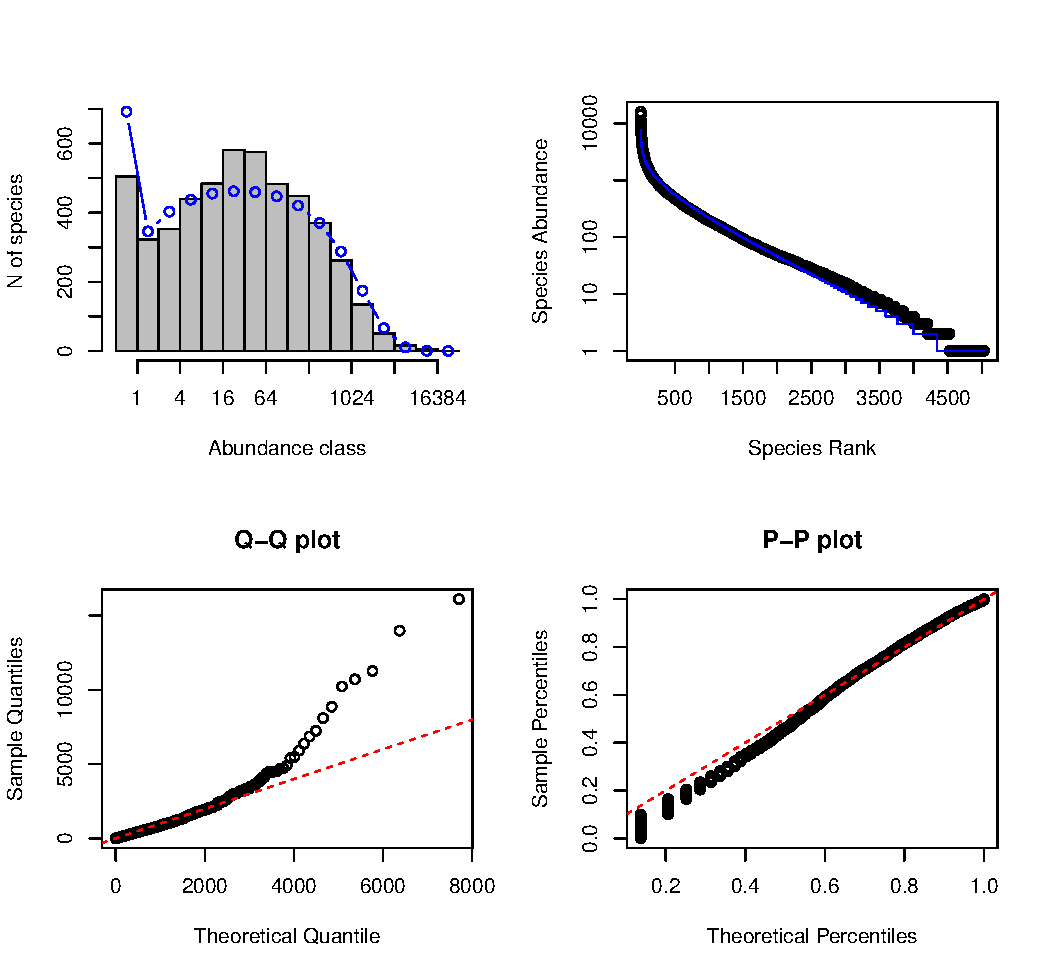
\includegraphics[width=\maxwidth]{figure/fit_ls-1} 

}



\end{knitrout}

\subsection*{Estimate of species richness}

Well, you have that stuck in your brain, I suppose. 
But just for the records:

 
\begin{knitrout}
\definecolor{shadecolor}{rgb}{0.969, 0.969, 0.969}\color{fgcolor}\begin{kframe}
\begin{alltt}
\hlstd{alpha} \hlkwb{<-} \hlkwd{coef}\hlstd{(y.ls)[[}\hlnum{2}\hlstd{]]}
\hlstd{(S.ls} \hlkwb{<-} \hlstd{alpha}\hlopt{*}\hlkwd{log}\hlstd{(}\hlnum{1} \hlopt{+} \hlstd{Tot.t}\hlopt{/}\hlstd{alpha))}
\end{alltt}
\begin{verbatim}
## [1] 13809.86
\end{verbatim}
\end{kframe}
\end{knitrout}

And here is the confidence interval for Fisher's $\alpha$ and the
interval for estimated total richness from these values

\begin{knitrout}
\definecolor{shadecolor}{rgb}{0.969, 0.969, 0.969}\color{fgcolor}\begin{kframe}
\begin{alltt}
\hlstd{(ls.ci} \hlkwb{<-} \hlkwd{confint}\hlstd{(y.ls))}
\end{alltt}
\begin{verbatim}
##    2.5 %   97.5 % 
## 638.9166 750.1000
\end{verbatim}
\begin{alltt}
\hlcom{## Estimated species richness for lower bound of alpha's IC}
\hlstd{ls.ci[}\hlnum{1}\hlstd{]}\hlopt{*}\hlkwd{log}\hlstd{(}\hlnum{1} \hlopt{+} \hlstd{Tot.t}\hlopt{/}\hlstd{ls.ci[}\hlnum{1}\hlstd{])}
\end{alltt}
\begin{verbatim}
##    2.5 % 
## 12782.17
\end{verbatim}
\begin{alltt}
\hlstd{ls.ci[}\hlnum{2}\hlstd{]}\hlopt{*}\hlkwd{log}\hlstd{(}\hlnum{1} \hlopt{+} \hlstd{Tot.t}\hlopt{/}\hlstd{ls.ci[}\hlnum{2}\hlstd{])}
\end{alltt}
\begin{verbatim}
##   97.5 % 
## 14886.17
\end{verbatim}
\end{kframe}
\end{knitrout}

\section*{Negative binomial}

Here I use the method proposed by \citet{tovo2017}. The first step is
to fit a negative binomial to the abundances in the sample.
I did that with the \emph{VGAM} package (as the authors did)
and also with the \emph{sads} package. 
The results were similar, and the fit looks identical to
those provided by the log-series (but has much lower AIC value, see below).

 
\begin{knitrout}
\definecolor{shadecolor}{rgb}{0.969, 0.969, 0.969}\color{fgcolor}\begin{kframe}
\begin{alltt}
\hlcom{## With VGAM}
\hlstd{y.nb} \hlkwb{<-} \hlkwd{vglm}\hlstd{(y} \hlopt{~} \hlnum{1}\hlstd{, posnegbinomial)}
\hlcom{## With sads}
\hlstd{y.nb2} \hlkwb{<-} \hlkwd{fitnbinom}\hlstd{(y,} \hlkwc{start.value}\hlstd{=}\hlkwd{c}\hlstd{(}\hlkwc{size}\hlstd{=}\hlnum{0.3}\hlstd{,} \hlkwc{mu}\hlstd{=}\hlkwd{mean}\hlstd{(y)))}
\hlcom{## Comparing: }
\hlkwd{exp}\hlstd{(}\hlkwd{coef}\hlstd{(y.nb))}
\end{alltt}
\begin{verbatim}
## (Intercept):1 (Intercept):2 
##   48.96347392    0.04048581
\end{verbatim}
\begin{alltt}
\hlkwd{coef}\hlstd{(y.nb2)}
\end{alltt}
\begin{verbatim}
##        size          mu 
##  0.04153996 50.08844429
\end{verbatim}
\end{kframe}
\end{knitrout}

\begin{knitrout}
\definecolor{shadecolor}{rgb}{0.969, 0.969, 0.969}\color{fgcolor}\begin{kframe}
\begin{alltt}
\hlkwd{par}\hlstd{(}\hlkwc{mfrow}\hlstd{=}\hlkwd{c}\hlstd{(}\hlnum{2}\hlstd{,}\hlnum{2}\hlstd{))}
\hlkwd{plot}\hlstd{(y.nb2)}
\hlkwd{par}\hlstd{(}\hlkwc{mfrow}\hlstd{=}\hlkwd{c}\hlstd{(}\hlnum{1}\hlstd{,}\hlnum{1}\hlstd{))}
\end{alltt}
\end{kframe}

{\centering 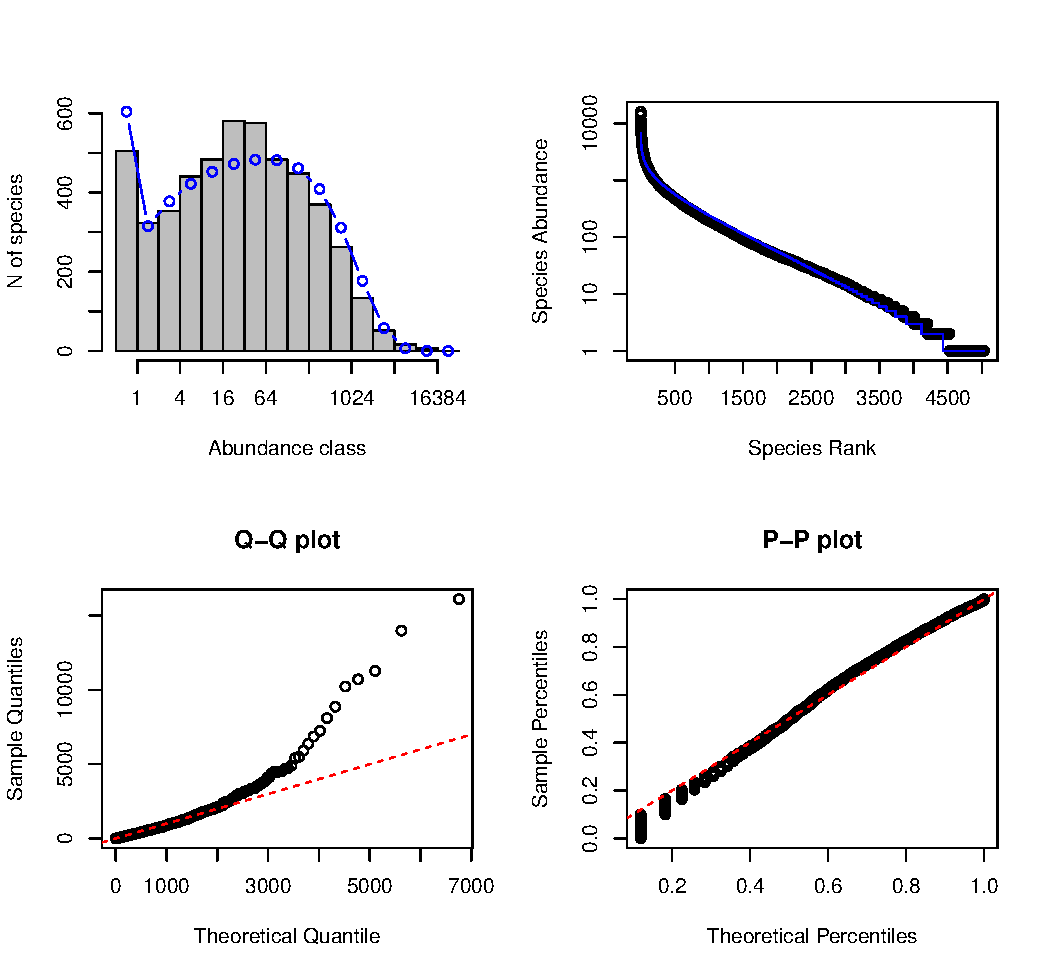
\includegraphics[width=\maxwidth]{figure/nb_plots-1} 

}



\end{knitrout}


\subsection*{Estimate of  species richness}

Following the recipe of \citet{tovo2017}:

 
\begin{knitrout}
\definecolor{shadecolor}{rgb}{0.969, 0.969, 0.969}\color{fgcolor}\begin{kframe}
\begin{alltt}
\hlstd{cf.nb} \hlkwb{<-} \hlkwd{coef}\hlstd{(y.nb2)}
\hlstd{csi.p} \hlkwb{<-} \hlkwd{unname}\hlstd{(cf.nb[}\hlnum{2}\hlstd{]}\hlopt{/}\hlstd{(}\hlkwd{sum}\hlstd{(cf.nb)))}
\hlstd{csi} \hlkwb{<-} \hlstd{csi.p}\hlopt{/}\hlstd{(p1}\hlopt{+}\hlstd{(}\hlnum{1}\hlopt{-}\hlstd{p1)}\hlopt{*}\hlstd{csi.p)}
\hlcom{## Estimated number of species }
\hlstd{S.est} \hlkwb{<-} \hlstd{Sobs}\hlopt{*}\hlstd{(}\hlnum{1}\hlopt{-}\hlstd{(}\hlnum{1}\hlopt{-}\hlstd{csi)}\hlopt{^}\hlstd{cf.nb[}\hlnum{1}\hlstd{])} \hlopt{/} \hlstd{(}\hlnum{1}\hlopt{-}\hlstd{(}\hlnum{1}\hlopt{-}\hlstd{csi.p)}\hlopt{^}\hlstd{cf.nb[}\hlnum{1}\hlstd{])}
\hlkwd{unname}\hlstd{(S.est)}
\end{alltt}
\begin{verbatim}
## [1] 11038.67
\end{verbatim}
\end{kframe}
\end{knitrout}

I did a simple function to automate the calculations and to return
the confidence intervals, based on the confidence intervals of the 
coefficients of the NB fit (see file \code{functions.R})

 
\begin{knitrout}
\definecolor{shadecolor}{rgb}{0.969, 0.969, 0.969}\color{fgcolor}\begin{kframe}
\begin{alltt}
\hlkwd{tovo}\hlstd{(}\hlkwc{fit} \hlstd{= y.nb2,} \hlkwc{p} \hlstd{= p1,} \hlkwc{CI}\hlstd{=}\hlnum{TRUE}\hlstd{)}
\end{alltt}
\begin{verbatim}
## Estimated species richness: 11038.67 
##  95% CI: 10328.09 - 11977.2
\end{verbatim}
\end{kframe}
\end{knitrout}


\section*{Model selection}

Among the three models, the Negative Binomial
provides the best fit:

 
\begin{knitrout}
\definecolor{shadecolor}{rgb}{0.969, 0.969, 0.969}\color{fgcolor}\begin{kframe}
\begin{alltt}
\hlkwd{AICtab}\hlstd{(pln, y.nb2, y.ls,} \hlkwc{base}\hlstd{=}\hlnum{TRUE}\hlstd{)}
\end{alltt}
\begin{verbatim}
##       AIC     dAIC    df
## y.nb2 54530.9     0.0 2 
## y.ls  54557.5    26.6 1 
## pln   54577.6    46.6 2
\end{verbatim}
\end{kframe}
\end{knitrout}

\section*{Parametric estimates from occupancies}

Here goes a quick exploration of models for the distribution of
occupancies (that is, the proportion of plots in which each species
has been recorded). Such distribution captures a bit of
the spatial aggregation of species \footnote{check if what has already been done with these distributions; maybe we can call them SODs (Species Occupancy Distributions). Moreover, following core-satellite hypothesis, occupancies should correlate with abundances and them we might think on modelling a bivariate SAD x SOD distribution.}. 

I tried two tentative approaches.
The first one was to calculate the empirical occupancies (that is, the proportion
of plots in which each species has been recorded) and then I fitted
a beta distribution to these values. 
To take into account undetected species I tried to truncate this
continuous distribution at different points.

The second approach was to fit the distribution
of frequencies (the number of plots out of the total of 1945
in which each species has been recorded) to
a beta-binomial distribution. Because this is a discrete distribution, 
truncation is at a single point (species with zero frequency in the sample).

In both cases I assumed that the occupancies of the species
follow a beta distribution, and that the observed frequencies were
the result of independent 1945 trials for each species, in which
the number of occupied plots follow a binomial distribution. 
Hence the compound beta-binomial distribution that underlies both approaches.
With this distribution we can estimate the proportion of undetected species
and then the total number of species.

\subsection*{Truncated Beta distribution}

The beta distribution is used to describe a distribution of bounded
continuous variables like probabilities. We can think observed
occupancies as estimates of the probabilities of occurrence of each species
in a plot. 

Because species with low occupancy values have lower detectability,
the distribution should give more weight for the lower values of occupancies,
as they are underrepresented in the sample. 
A first-order approximation is to truncate the
beta distribution at 1/(number of plots). 

I then fitted the distribution of occupancies to beta distributions
without truncation and truncated at $0.1/$1945, $0.5/$1945 and $0.9$1945.
The code for fitting with maximum likelihood
is in the source file of this document.  
Below I show the QQplots of predicted x observed values,
which shows that truncation above $0.5/$1945 clearly
improves the fit:

\begin{knitrout}
\definecolor{shadecolor}{rgb}{0.969, 0.969, 0.969}\color{fgcolor}\begin{kframe}
\begin{verbatim}
##        s1        s2 
##  0.473385 23.882701
##         s1         s2 
##  0.3083174 17.9980203
##          s1          s2 
##  0.07090589 11.67846020
##           s1           s2 
## 5.217535e-05 1.086736e+01
\end{verbatim}
\end{kframe}
\end{knitrout}

\begin{knitrout}
\definecolor{shadecolor}{rgb}{0.969, 0.969, 0.969}\color{fgcolor}

{\centering 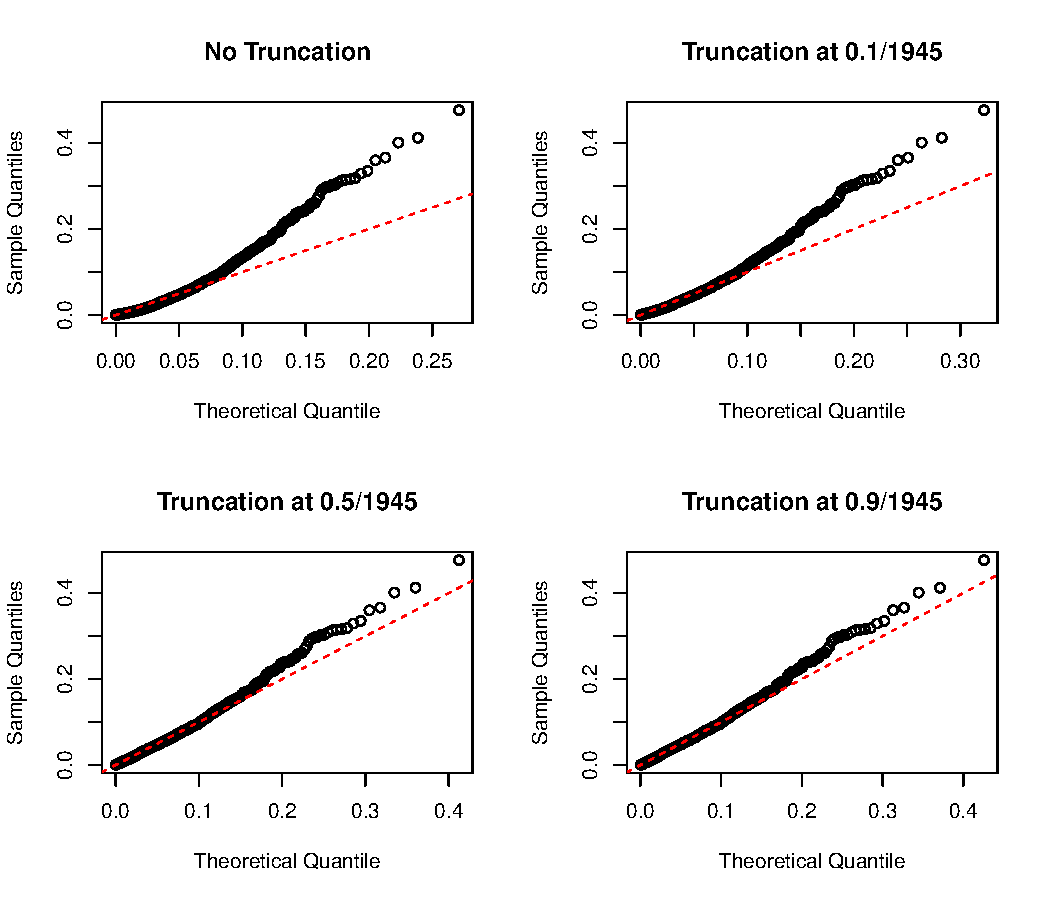
\includegraphics[width=\maxwidth]{figure/beta_qqplots-1} 

}



\end{knitrout}

And the model selection shows that the truncation at $0.9/$1945
provides a much better fit:

\begin{knitrout}
\definecolor{shadecolor}{rgb}{0.969, 0.969, 0.969}\color{fgcolor}\begin{kframe}
\begin{alltt}
\hlkwd{AICtab}\hlstd{(f.beta, f.betat.1, f.betat.5, f.betat.9)}
\end{alltt}
\begin{verbatim}
##           dAIC   df
## f.betat.9    0.0 2 
## f.betat.5 1112.7 2 
## f.betat.1 2528.3 2 
## f.beta    3270.3 2
\end{verbatim}
\end{kframe}
\end{knitrout}

\subsubsection*{Estimate of species richness}



If we assume that species occur in the plots
independently with different values of occupancies
(described by the beta distribution fitted above),
the distribution of frequencies (number of occupied plots) 
follows a \textbf{beta-binomial distribution}. Because species that
have not occurred in any plot are undetected, 
the beta-binomial distribution
of observed frequencies is truncated at zero. 
The full distribution nevertheless returns the probability
of zero frequency, which estimates the proportion of species
not recorded. With this and the number of observed species we
can estimate the total number of species. I did a function
to do this (see scripts at \texttt{functions.R}) and
got the following:

\begin{knitrout}
\definecolor{shadecolor}{rgb}{0.969, 0.969, 0.969}\color{fgcolor}
\begin{tabular}{l|r}
\hline
Truncation & Estimated richness\\
\hline
None & 5642\\
\hline
0.1/N plots & 6458\\
\hline
0.5/N plots & 16142\\
\hline
0.9/N plots & 18099397\\
\hline
\end{tabular}


\end{knitrout}

The distribution truncated at $0.9/$1945 gives unrealistic estimates,
so I'll follow with the model with truncation at $0.5/$1945.
With the likelihood surface we get an idea of likelihood interval:
%I get a likelihood interval for the richness estimated by this model of 13000--22200.

\begin{knitrout}
\definecolor{shadecolor}{rgb}{0.969, 0.969, 0.969}\color{fgcolor}

{\centering 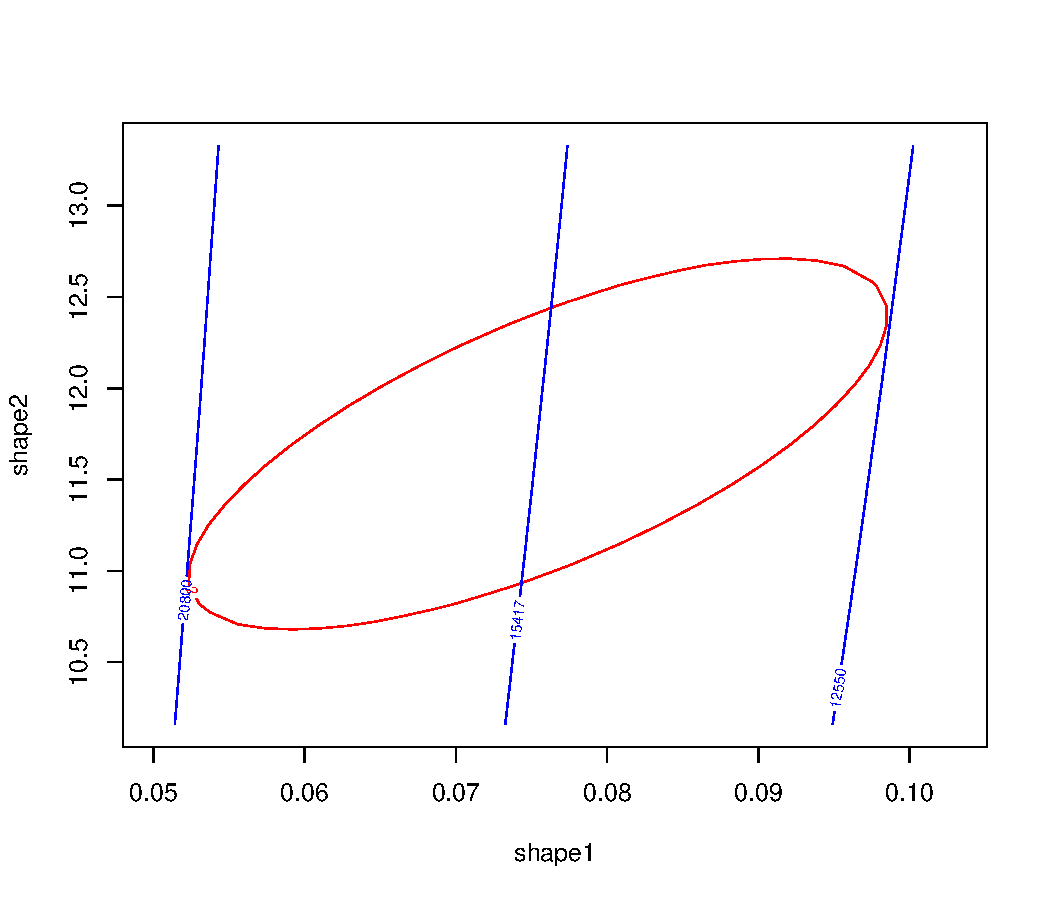
\includegraphics[width=\maxwidth]{figure/beta_likelihood_surface-1} 

}



\end{knitrout}

\subsection*{Truncated beta-binomial}



Another easy way to get species richness estimates
from the beta-binomial is to fit this distribution
directly to the observed frequencies.
This distribution is zero-truncated to account for
the unobserved species. In this case only the
binomial distribution that composes the beta-binomial
is truncated. To truncate also the beta compounding distribution
we would need Bayesian models.

With this model I got an estimated total richness of
\ensuremath{1.0081\times 10^{4}}, with an likelihood interval below:

\begin{knitrout}
\definecolor{shadecolor}{rgb}{0.969, 0.969, 0.969}\color{fgcolor}

{\centering 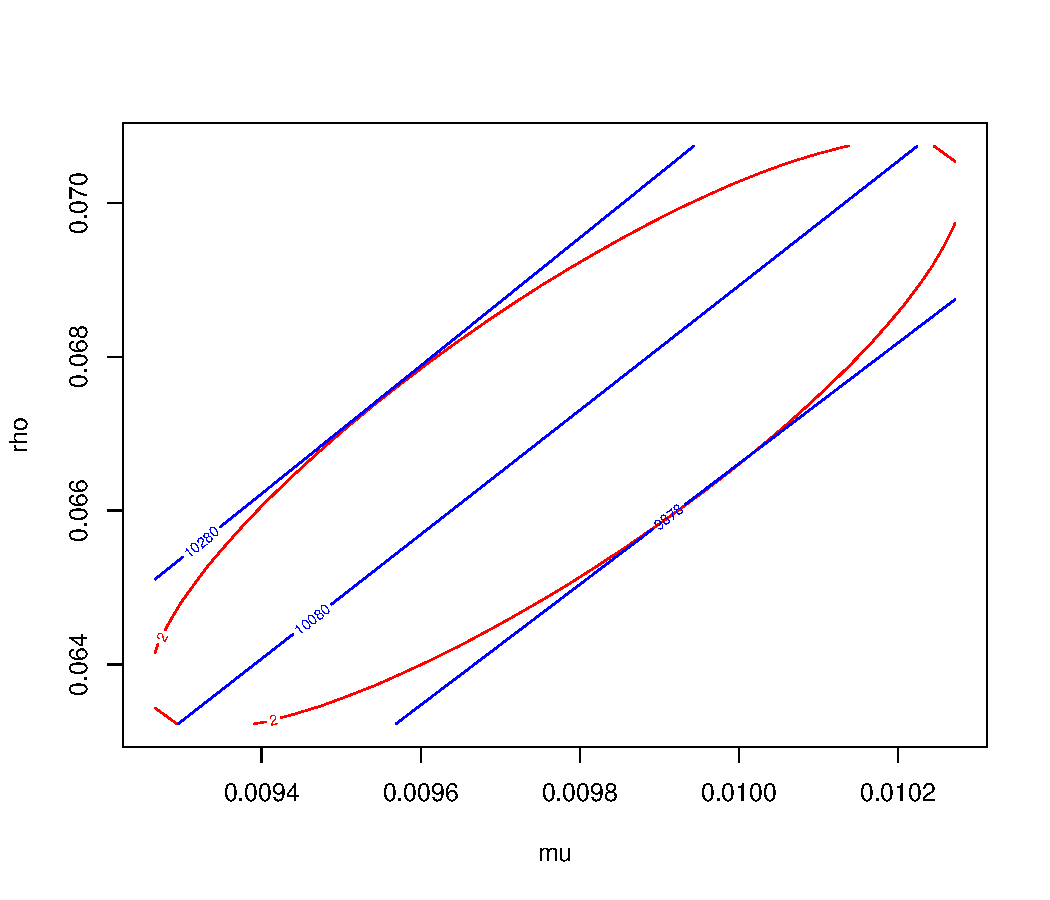
\includegraphics[width=\maxwidth]{figure/beta-binomial_likelihood_surface-1} 

}



\end{knitrout}

\section*{Non-parametric estimates}

Results of the non-parametric indices
available in the package \emph{SPECIES} \citep{SPECIES}.
All around ~5000 species.
%% Only the 'Penalized non-parametric maximum likelihood estimate'
%% from \citet{wang2005} is close the number of species recorded in Amazon. 
%% The other indices estimate  ~5000 species.

\begin{knitrout}
\definecolor{shadecolor}{rgb}{0.969, 0.969, 0.969}\color{fgcolor}\begin{kframe}
\begin{alltt}
\hlstd{Ab} \hlkwb{<-} \hlkwd{as.data.frame}\hlstd{(}\hlkwd{table}\hlstd{(dados}\hlopt{$}\hlstd{N.ind))}
\hlkwd{names}\hlstd{(Ab)} \hlkwb{<-} \hlkwd{c}\hlstd{(}\hlstr{"j"}\hlstd{,} \hlstr{"n_j"}\hlstd{)}
\hlstd{Ab}\hlopt{$}\hlstd{j} \hlkwb{<-} \hlkwd{as.integer}\hlstd{(}\hlkwd{as.character}\hlstd{(Ab}\hlopt{$}\hlstd{j))}
\hlcom{##jackknife method}
\hlstd{(Sj} \hlkwb{<-} \hlkwd{jackknife}\hlstd{(Ab,}\hlkwc{k}\hlstd{=}\hlnum{5}\hlstd{))}
\end{alltt}
\begin{verbatim}
## 
## Your specified order is larger than that determined by the test, 
## Therefore the order from the test is used.
## $JackknifeOrder
## [1] 2
## 
## $Nhat
## [1] 5737
## 
## $SE
## [1] 55.53377
## 
## $CI
##        lb   ub
## [1,] 5628 5846
\end{verbatim}
\begin{alltt}
\hlcom{##ACE coverage method}
\hlstd{(SChao92} \hlkwb{<-} \hlkwd{ChaoLee1992}\hlstd{(Ab,}\hlkwc{t}\hlstd{=}\hlnum{10}\hlstd{,} \hlkwc{method}\hlstd{=}\hlstr{"all"}\hlstd{))}
\end{alltt}
\begin{verbatim}
## $Nhat
## [1] 5399 5485
## 
## $SE
## [1] 33.21531 44.06319
## 
## $CI
##         lb   ub
## ACE   5334 5464
## ACE-1 5400 5573
\end{verbatim}
\begin{alltt}
\hlcom{##Chao1984 lower bound estimator}
\hlstd{(SChao84} \hlkwb{<-} \hlkwd{chao1984}\hlstd{(Ab))}
\end{alltt}
\begin{verbatim}
## $Nhat
## [1] 5441
## 
## $SE
## [1] 47.05694
## 
## $CI
##        lb   ub
## [1,] 5358 5544
\end{verbatim}
\begin{alltt}
\hlcom{##Chao and Bunge coverage-duplication method}
\hlstd{(SChaoB} \hlkwb{<-} \hlkwd{ChaoBunge}\hlstd{(Ab,}\hlkwc{t}\hlstd{=}\hlnum{10}\hlstd{))}
\end{alltt}
\begin{verbatim}
## $Nhat
## [1] 5542
## 
## $SE
## [1] 55.42057
## 
## $CI
##        lb   ub
## [1,] 5435 5652
\end{verbatim}
\begin{alltt}
\hlcom{##Penalized NPMLE method}
\hlstd{(SNPMLE} \hlkwb{<-} \hlkwd{pnpmle}\hlstd{(Ab,}\hlkwc{t}\hlstd{=}\hlnum{15}\hlstd{))}
\end{alltt}
\begin{verbatim}
## Method: Penalized NPMLE method by  Wang and Lindsay 2005. 
## 
##         MLE=                                5551 
##         Estimated zero-truncated Poisson mixture components:       
##         p=                                  0.9153796 2.048484 4.198693 9.778435 
##         pi=                                 0.3390338 0.0835869 0.2598503 0.317529
## $Nhat
## [1] 5551
\end{verbatim}
\begin{alltt}
\hlcom{##Unconditonal NPMLE method}
\hlstd{(SUNPMLE} \hlkwb{<-}\hlkwd{unpmle}\hlstd{(Ab,}\hlkwc{t}\hlstd{=}\hlnum{10}\hlstd{))}
\end{alltt}
\begin{verbatim}
## Method: Unconditional NPMLE method by Norris and Pollock 1996, 1998, 
##         using algorithm by Wang and Lindsay 2005: 
## 
##         MLE=                                5608 
##         Estimated Poisson mixture components:       
##         p=                                  0.370657 1.411825 6.183764 
##         pi=                                 0.1811724 0.4804983 0.3383293
## $Nhat
## [1] 5608
\end{verbatim}
\begin{alltt}
\hlcom{##Poisson-compound Gamma method}
\hlstd{(SPG} \hlkwb{<-} \hlkwd{pcg}\hlstd{(Ab,}\hlkwc{t}\hlstd{=}\hlnum{20}\hlstd{))}
\end{alltt}
\begin{verbatim}
## Method: Poisson-Compound Gamma method by Wang 2010. 
## Alpha grid used: 1 2 3 4 5 6 7 8 9 10 . 
## 
##         MLE=                                5576 
##         Selected alpha model:               Inf 
##         Estimated Gamma components:         
##         p=                                  0.734205 2.246373 6.79769 14.67896 
##         pi=                                 0.2218206 0.2631206 0.286423 0.2286358
## $Nhat
## [1] 5576
## 
## $AlphaModel
## [1] Inf
\end{verbatim}
\end{kframe}
\end{knitrout}

\section*{Wrap up}

\subsection*{Findings}
\begin{itemize}
\item There is a gap between the estimates, rather than a more uniform spread over the range of values. We have a cluster of estimates around 5000-6000 and other around or above the known number of species.
\item Using a strict approach of selecting the best SAD model with AIC, negative binomial wins. As noted by \citet{tovo2017}, NB provides a lower total richness estimate compared to Log-series. But now it is still a realistic value (\ensuremath{1.1038668\times 10^{4}}). The diagnostic plots show that is so because LS overestimate singletons more than NB. If we go for NB we would check if/how to make the hypothetical SAD for the whole Amazonia from a Negative Binomial, as the codes by Steege et al. do.
\item The realistic estimates (that is, above the known number of species)  
  came from methods that
  approximate some  effect of a large beta-diversity. 
  Such beta-diversity effect is approximated in different ways.
  Log-series assumes an open metacommunity with an infinite number of species,
  negative binomial describes SADs with a variance higher than those expected
  by an independent distribution of species, beta-binomial models
  capture spatial aggregation of species.
\end{itemize}

\subsection*{Open questions}

\begin{itemize}
\item Which models to include?
  \begin{itemize}
  \item I would not use the 1st method to estimate S from Poisson-Lognormal, nor the truncated beta method. Agree?
  \item On the other hand, not so sure if we should include truncated beta-binomial. \textbf{Pros}: raises an simple, alternative way to estimate (occupancy-based); realistic estimates based on some assumption of beta-diversity. \textbf{Cons}: shift the focus from SADs (best keep for another paper?); need to search in the literature to check if/how this method has already been used.
  \end{itemize}
\item Keep the estimation based the reconstruction of the regional SAD? If so, try to do that for negative binomial? If we stick to the current reconstruction based on LS, how to deal with the better performance of NB from model selection?
\end{itemize}

\section*{More (and some redundant) thoughts}

Oldies, kept for the records

I can see a paper that reviews comprehensively the species richness estimates we can get from this data. Of course one important information is the known number of species recorded in the region. There is a gap between the estimates, rather than a more uniform spread over the range of values. We have a cluster of estimates around 5000-6000 and other around the known number of species. Another idea is to do the same for Mata Atlantica.  A nice main figure would be a point-and-error-bars of all estimates for both ecorregions.

The estimates provided by non-parametric and
also the parametric methods with strong assumptions of random and independent dispersion of species
across space (which implies in describing the plots as Poisson samples) were
consistently below the number of species currently recorded for the Amazon.

On the other hand, parametric estimates based on models that
approximates some  effect of a large beta-diversity 
provided consistently larger
values, which encompassed the known number of species. 
Such beta-diversity effect is approximated in different ways.
Log-series assumes an open metacommunity with an infinite number of species,
negative binomial describes SADs with a variance higher than those expected
by an independent distribution of species, and beta and beta-binomial models
capture spatial aggregation of species. 
%% Still to be checked,
%% the only non-parametric estimate that was above 10,000 has also a similar 
%% effect by allowing a different detectability for each species \citep{wang2005}.
I think that the key message here 
is that beta-diversity matters a lot to get a better estimate. And also
that those models that performed better are still rough approximations.

Also, I think that the comparison of the saturation curves of the estimators you did 
for the Amazon is nice. 
Many of them seem to stabilize well below the known number of species, 
while others do show an increasing trend. I think this may be valuable
to discuss the quality of the estimates available for the Amazon. 
I would not venture in general evaluations of the estimators because
there is already a ton of papers about that, so I think we do not
need the simulated data.

%% Finally, I found interesting that
%% some models provided a good fit
%% to a distribution but did not provide a good estimate of species richness.
%% The obvious explanation is that the approximation any model does
%% may break down when you use it in extrapolations. But as obvious it may sound
%% I think it is an important issue concerning the estimation of species richness.


\subsection*{Next steps}

Not sure if for the same paper, but I would proceed with the idea of a model that improves
assumptions about a large beta-diversity. 
My first guess is a minimum model that assumes different degrees
of aggregation for each species. My first choice is a compound Negative binomial-Lognormal
distribution. This is hard to fit by traditional methods, but it is doable with 
simulation and ABC (Approximate Bayesian Computation). To parameterize simulations
we can use the empirical matrix of species x sites. 
I started to work in this idea with Renato and I have some preliminary R codes
of a bootsrap estimator. The \emph{SADISA} package uses a similar approach (using the information of 
replicate samples from the same metacommunity).

A related topic is the idea of SOD's (Species Occupancies Distributions),
which depends of checking if we are not reinventing the weel. But I think
that combining SODs and SADs in a bivariate model has not been fully explored
yet.

\bibliography{/home/paulo/work/resources/bib/geral.bib}

\end{document}
